\documentclass[a4paper,12pt,titlepage,floatssmall]{article}

% Page geometry's formatting
\usepackage[left=3.5cm,right=2.5cm,top=2.5cm,bottom=2.5cm]{geometry}
\usepackage{indentfirst}
\usepackage{placeins}
\usepackage{float}
% Language-specific settings
\usepackage[T1]{fontenc}
\usepackage[utf8]{inputenc}
\usepackage[polish]{babel}
\usepackage{polski}
% Elements' embedding
\usepackage{listings}
\usepackage{graphicx}
\usepackage{hyperref}
% Text-formatting
\usepackage[autostyle]{csquotes}
\usepackage{moresize}
\usepackage{amsmath}
% Miscellaneous
\usepackage[backend=biber,style=ieee]{biblatex}
\usepackage[enable]{easy-todo}
\usepackage{lipsum}


% ============================================================================================================== %
% ----------------------------------------------- Configuration ------------------------------------------------ %
% ============================================================================================================== %

% Bibliography file
\addbibresource{tex/bibliography.bib}

% Unordered list
\renewcommand{\labelitemi}{\textbullet}

% Removing clearpage after abstract
\makeatletter
\renewenvironment{abstract}{%
      %\titlepage
      %\null\vfil
      \@beginparpenalty\@lowpenalty
      \small
      \begin{center}%
        \bfseries \abstractname
        \@endparpenalty\@M
      \end{center}\quotation}%
     {\quotation\par%\vfil\null\endtitlepage
     }
\makeatother


% ============================================================================================================== %
% --------------------------------------------- Macrodefinitions ----------------------------------------------- %
% ============================================================================================================== %

% Redefininiton of the title page
\renewcommand{\maketitle}{
\begin{titlepage}
    \vfill
    \begin{center}
        \begin{figure}
            \centering
            
\includegraphics[scale=0.9]{img/header.png}
            \vspace{0.5cm}
        \end{figure}
    \end{center}
    \vspace{2cm}
    \begin{center}
        {\HUGE {\bf Sieci neuronowe}}\\
        \vspace {0.4cm}
        {\Large {(projekt)}}
    \end{center}
    \vspace{4cm}
    \begin{center}
        {\bf \LARGE Wykorzystanie sieci VGG19 \\do~klasyfikacji owoców}
        \vspace{3cm}
    \end{center}
    \vfill
    \begin{center}
        {\bf \normalsize Drelich Ewelina, Dziurlikowski Krzysztof, \\Pawlak Iga, Pierczyk Krzysztof}
    \end{center}
    \vfill
    \begin{center}
        \large{Warszawa, \today \par}
    \end{center}
\end{titlepage}
}


% ============================================================================================================== %
% --------------------------------------------------- Text ----------------------------------------------------- %
% ============================================================================================================== %

\begin{document}
    
% Title
\maketitle

% Table of content
% \tableofcontents

% Abstract
\begin{abstract}

    Sztuczne sieci neuronowe na stałe zadomowiły się w~dziedzinie, którą dzisiaj powszechnie określamy mianem sztucznej inteligencji. Algorytmy tworzone przez firmy jak Google potrafią już same uczyć się operowania w~tak złożonych grach jak szachy czy Starcraft II znacząco przewyższając wynikami ludzi \cite{mu_zero}. Coraz częściej pojawiają się również w~bardziej egzotycznych obszarach sterując balonami stratosferycznymi \cite{baloons} czy przewidując struktury przestrzenne długich łańcuchów aminokwasowych \cite{proteins}.
    
    Jednym z~klasycznych zastosowań sieci neuronowych jest klasyfikacja obrazów. Wśród najpowszechniej używanych w~tym celu architektur znajduje się od dłuższego czasu zaproponowana w~2014 roku \textit{VGG}. Niniejsza praca skupia się na jednym z~wariantów tego modelu -~VGG19~- analiząc jego możliwości w~kontekście klasyfikacji obrazów owoców ze zbioru \textit{Fruits-360}. Pierwsze trzy rozdziały stanowią opis postawionego problemu, wykorzystanej architektury oraz zbioru danych. Rozdział 4~opisuje przypadki uczenia klasyfikatorów typu perceptronowego oraz SVM bazujących na cechach generowanych przez warstwy splotowe sieci VGG19 uprzednio wytrenowanej na zbiorze \textit{ImageNet}. Następnie przedstawiony został trening części klasyfikującej (typu perceptronowego) wraz z~częścią lub wszystkimi warstawmi splotowymi. Przedostatni rozdział zgłębia analizę wytrenowanych sieci wykorzystując techniki wizualizacji obszarów uwagi oraz stopnia aktywacji poszczególnych warstw sieci.

\end{abstract}

% Chapters
\section{Analiza zadania}

\section{Architektura VGG19}

\section{Zbiór danych}

W~projekcie wykorzystana została baza danych \textbf{Fruits-360} \cite{fruits-360}, która inkorporuje zbiór ponad 90 tys. zdjęć owoców podzielonych na 131 klas. Zdjęcia dostarczone są w~formacie JPEG, a~ich wielkość została ustandaryzowana do wymiaru $100\times100$ pikseli. Warto nadmienić, że różne warianty tych samych gatunków owoców zostały umieszczone w~oddzielnych klasach. Dane zostały podzielone przez autorów na dwa podzbiory: \textit{Training} (67692 zdjęć) i \textit{Test} (22688 zdjęć).

\subsection{Potok}

\vspace{0.5cm}
\begin{figure}[h]
    \centering
    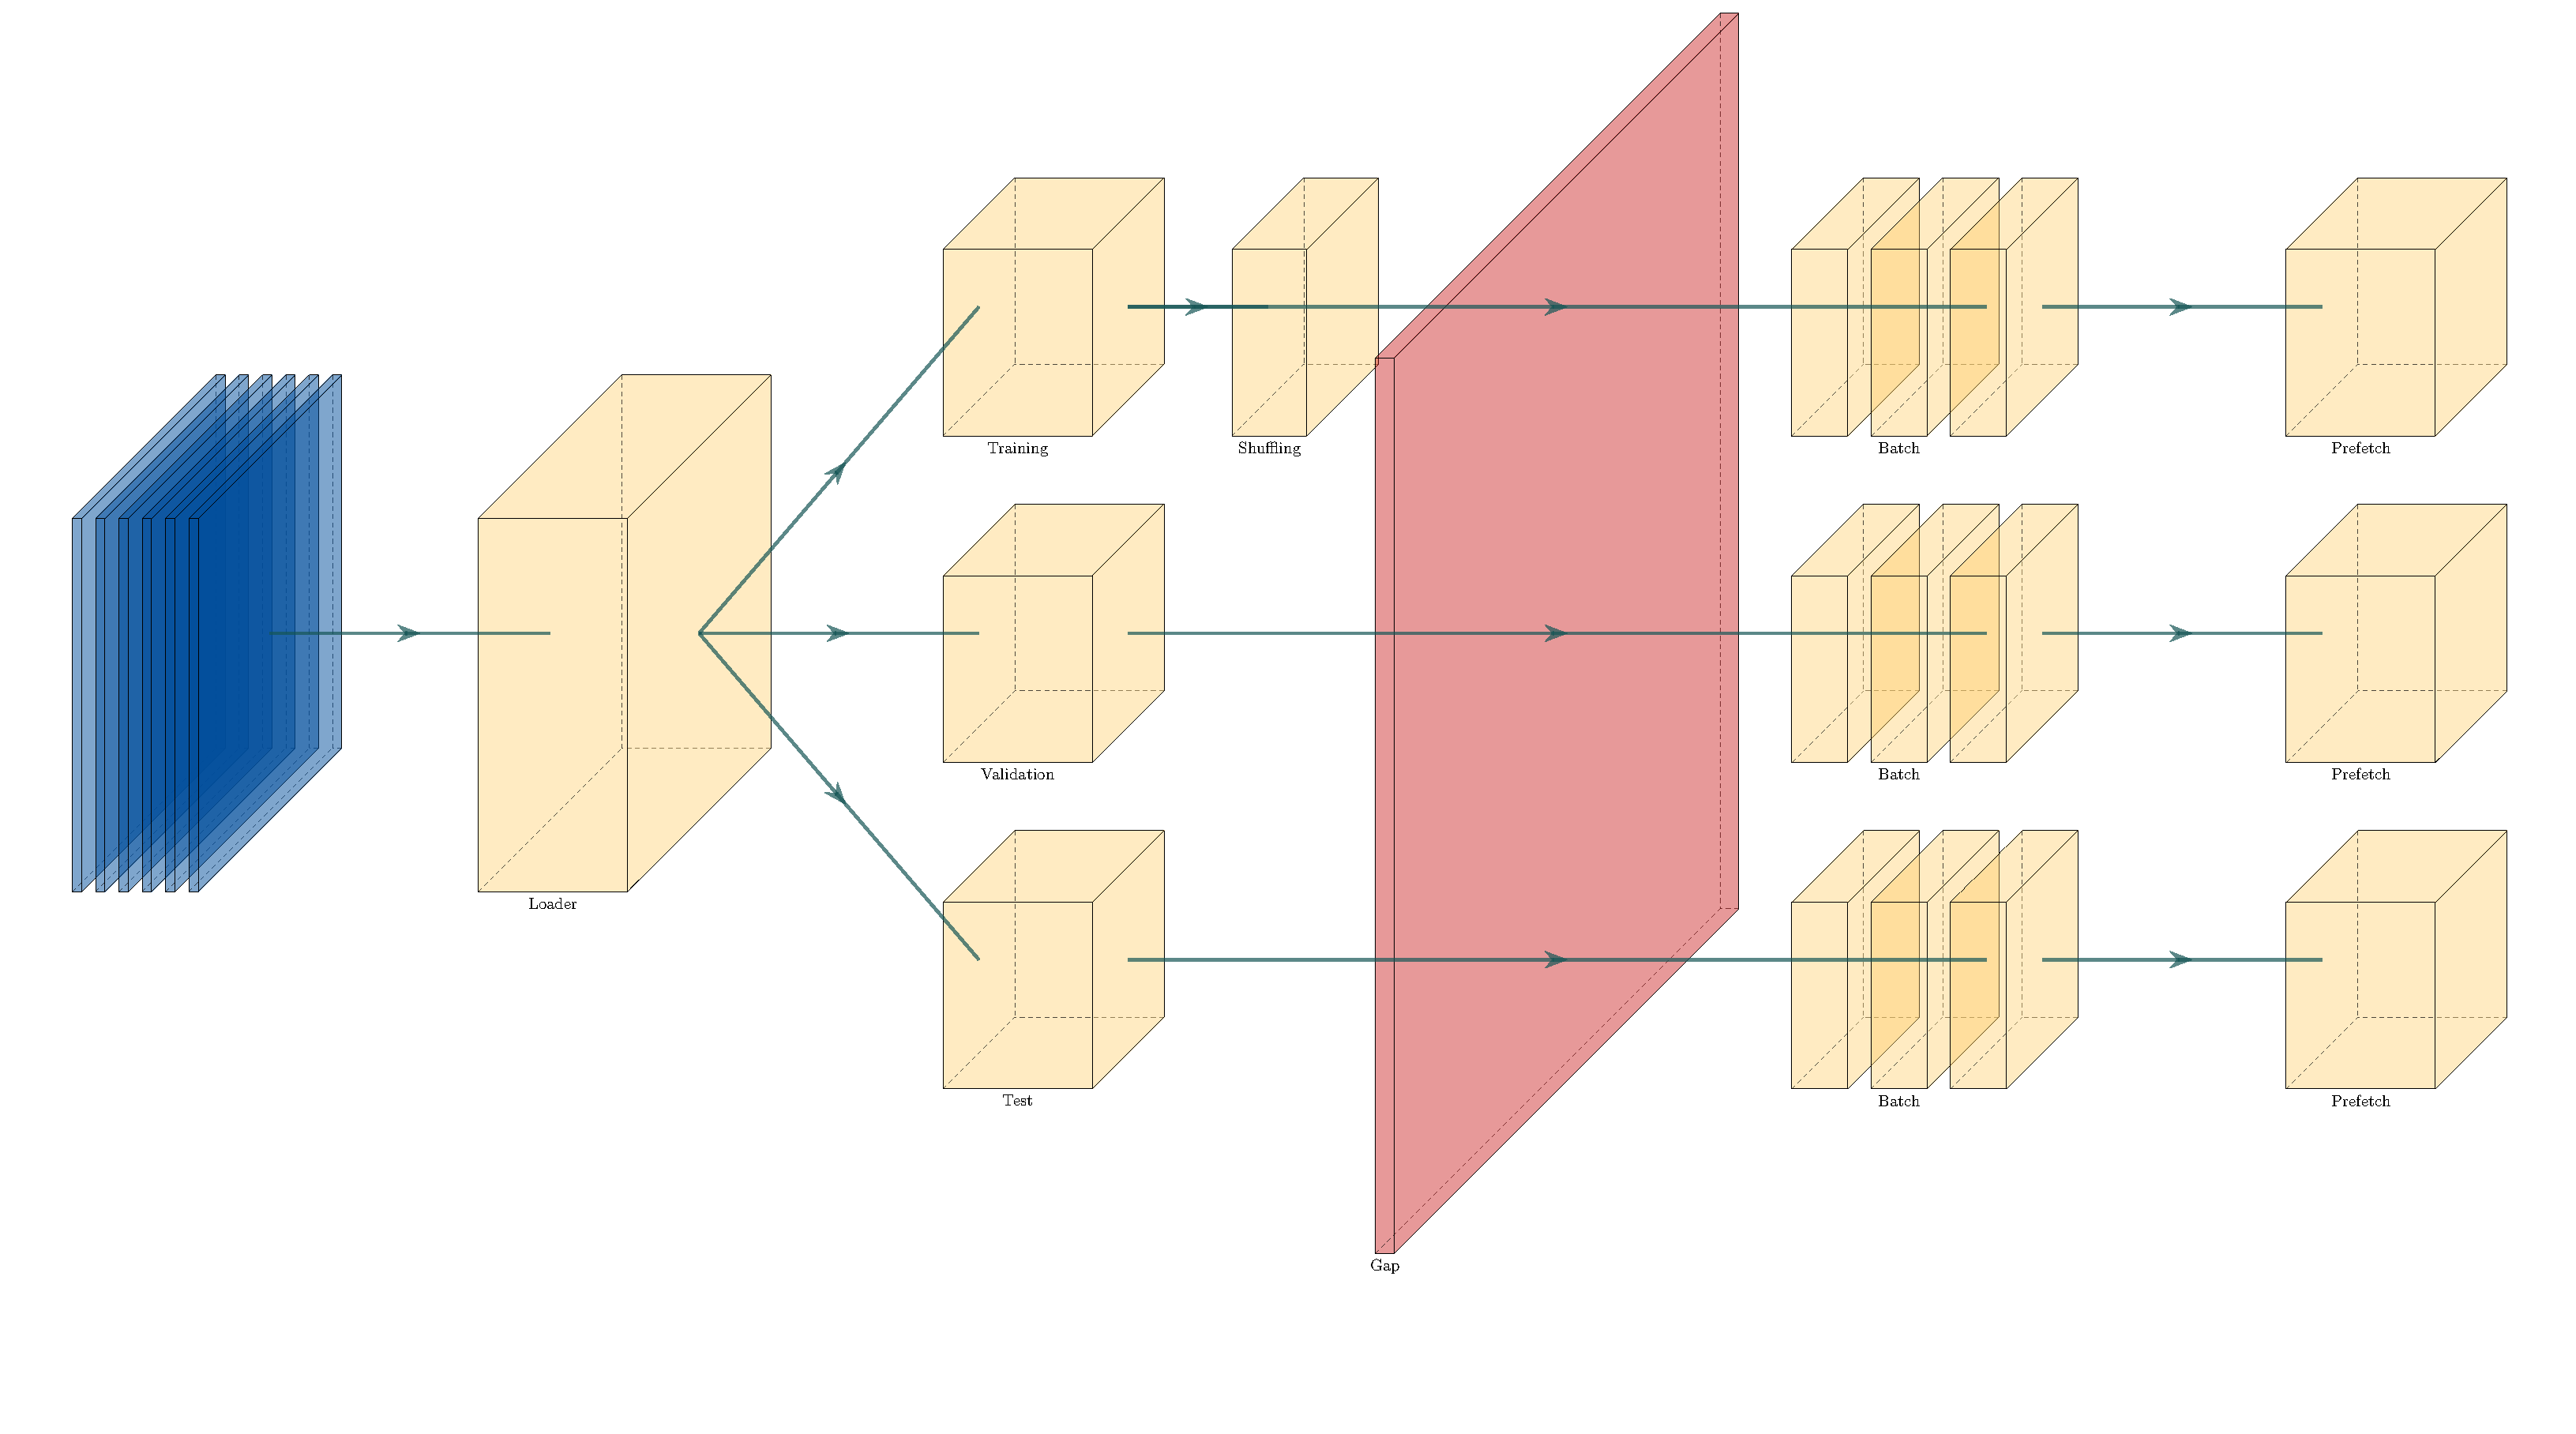
\includegraphics[scale=0.2]{img/pipe.pdf}
    \label{pipe_img}
    \caption{Struktura potoku danych wejściowych}
\end{figure}
\vspace{0.5cm}

Prace nad projektem rozpoczęto od wyboru bibliotek dostarczających zestaw podstawowych narzędzi uczenia maszynowego. Decyzja padła na popularny framework \textit{Tensorflow}, dzięki któremu możliwe było przygotowanie wygodnego, wysoce konfigurowalnego potoku danych wejściowych. Wykorzystanie \textit{tf.data} API pozwoliło na dynamiczne ładowanie danych do pamięci, co znacznie zredukowało jej zużycie  w~procesie uczenia. Możliwość zrównoleglenia tego procesu względem obliczeń wykonywanych na procesorze graficznym usunęła występujące początkowo wąskie gardło w~postaci procesu przenoszenia danych z~pamięci operacyjnej do VRAMu. Całość rozwiązania została zamknięta w~postaci klasy, której parametry mogłą być ustalane z~poziomu plików konfiguracyjnych. Takie podejście wyeliminowało potrzebę ingerowania w~kod źródłowy na etapie eksploatacji potoku. 

Rys. \ref{pipe_img} przedstawia graficzną reprezentację przepływu danych. Na wejściu następuje przydzielenie danych do trzech zbiorów. Podzbiór \textit{Training} jest w całości wykorzystywany jako zbiór treningowy. Z~kolei \textit{Test} \textbf{dzielony jest w~stosunku $1:1$} na dane walidacyjne i~testowe. W~kolejnym kroku nastepuje losowe przemieszanie danych treningowych. Obszar zaznaczony na rysunku na czerwono oznacza lukę. W~tym miejscu na zbiory można nałożyć arbitralne modyfikacje, co wykorzystywane jest na etapie augmentacji. Następnie wszystkie zbiory zostają podzielone na porcje (ang. \textit{mini-batches}). Ostatecznie część danych zostaje pobrana do bufora w~pamięci operacyjnej (faza \textit{prefetch}).
\subsection{Augmentacja}


\section{Klasyfikatory}

\subsection{Klasyfikator perceptronowy}

\subsection{Maszyna Wektorów Wspierających}

\subsection{Porównanie wyników}


\section{Sieci głębokie}

\subsection{Uczenie ostatniej warstwy splotowej}

\subsection{Uczenie dwóch ostatnich warstw splotowych}

\subsection{Przypadek pełnej sieci}

\subsection{Przypadek sieci o uproszczonej strukturze}

\subsection{Porównanie wyników}


\section{Wizualizacja}

\subsection{Klasyfikator perceptronowy}

\subsection{Maszyna Wektorów Wspierających}

\subsection{Uczenie ostatniej warstwy splotowej}

\subsection{Uczenie dwóch ostatnich warstw splotowych}

\subsection{Przypadek pełnej sieci}

\subsection{Przypadek sieci o uproszczonej strukturze}

\subsection{Porównanie wyników}


\section{Podsumowanie}


% Bibliography
\clearpage
\printbibliography

\end{document}


